\chapter{\ifproject%
\ifcpe โครงสร้างและขั้นตอนการทำงาน\else Project Structure and Methodology\fi
\else%
\ifcpe โครงสร้างของโครงงาน\else Project Structure\fi
\fi
}


\makeatletter

% \renewcommand\section{\@startsection {section}{1}{\z@}%
%                                    {13.5ex \@plus -1ex \@minus -.2ex}%
%                                    {2.3ex \@plus.2ex}%
%                                    {\normalfont\large\bfseries}}

\makeatother
%\vspace{2ex}
% \titleformat{\section}{\normalfont\bfseries}{\thesection}{1em}{}
% \titlespacing*{\section}{0pt}{10ex}{0pt}
ในบทนี้จะกล่าวถึงผลสรุปจากการสํารวจความคิดเห็นของนักศึกษาเกี่ยวกับตารางสอบปลายภาค ข้อมูลที่จำเป็นต้องใช้สำหรับการพัฒนาโปรแกรม รวมถึงโครงสร้างข้อมูลรับเข้าและข้อมูลส่งออกของโปรแกรม
ซึ่งจากความต้องการพัฒนาระบบจัดตารางสอบปลายภาคเพื่อให้นักศึกษามีอิสระในการเลือกลงทะเบียนเรียนมากขึ้นดังที่กล่าวในตอนที่ \ref{sec:project_rationale} เราจึงต้องการทราบความคิดเห็นของนักศึกษาในมหาวิทยาลัยเชียงใหม่เกี่ยวกับตารางสอบปลายภาค 
ทำให้เราได้จัดทำแบบสอบถามขึ้นเพื่อสอบถามความคิดเห็นของนักศึกษามหาวิทยาลัยเชียงใหม่ ทั้งนักศึกษาปัจจุบันและนักศึกษาที่สำเร็จการศึกษาแล้ว ว่ามีความคิดเห็นอย่างไรกับตารางสอบปลายภาคในปัจจุบัน และหากเลือกได้อยากจะสอบในช่วงเวลาใดบ้าง ๆ ในตารางเวลาของสัปดาห์ที่จัดสอบ 
โดยจะพยายามนำข้อมูลที่ได้มาใช้ในการอ้างอิงเพื่อออกแบบอัลกอริทึมสำหรับประมวลผลหาวิธีการจัดตารางสอบที่เหมาะสมที่สุดที่เป็นไปได้สำหรับนักศึกษาทุกคน

\section{การเก็บข้อมูล}
\subsection{การสำรวจความคิดเห็นของนักศึกษาเกี่ยวกับตารางสอบปลายภาค}
\label{sec:collecting_data}
จากผลสำรวจของแบบสอบถามเกี่ยวกับตารางสอบปลายภาคของมหาวิทยาลัยเชียงใหม่ โดยขอความร่วมมือนักศึกษาในมหาวิทยาลัย
ทั้งนักศึกษาที่กำลังศึกษาอยู่และทั้งที่สำเร็จการศึกษาไปแล้ว เพื่อให้ช่วยตอบแบบสอบถามความคิดเห็นเกี่ยวกับ ข้อดี ข้อเสีย ความพึงพอใจในตารางสอบของตนเอง
รวมถึงปัญหาเกี่ยวกับตารางสอบปลายภาคที่เคยพบหรือได้รับผลกระทบโดยตรง โดยจากผลการสำรวจกลุ่มสำรวจจำนวน 95 คน สามารถแบ่งผู้ตอบแบบสอบถามตามระดับการศึกษาได้ 5 ระดับดังกราฟที่ \ref{fig:academic_year} โดยมีจำนวนดังนี้
\begin{multicols}{2}
\begin{itemize}
  \item ชั้นปีที่ 1 จำนวน 14 คน
  \item ชั้นปีที่ 2 จำนวน 27 คน
  \item ชั้นปีที่ 3 จำนวน 11 คน
  \item ชั้นปีที่ 4 จำนวน 38 คน
  \item มากกว่าชั้นปีที่ 4 จำนวน 2 คน
  \item สำเร็จการศึกษาแล้ว จำนวน 3 คน
\end{itemize}
\end{multicols}
\begin{figure}
  \begin{center}
    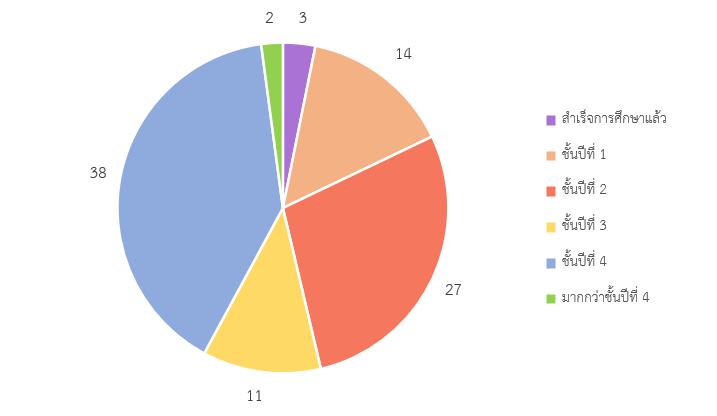
\includegraphics[width=4in]{images/group_by_academic_year.png}
  \end{center}
  \caption[จำนวนผู้ตอบแบบสอบถามแบ่งตามชั้นปีที่ศึกษา]{จำนวนผู้ตอบแบบสอบถามแบ่งตามชั้นปีที่ศึกษา}
  \label{fig:academic_year}     
\end{figure}
และหากแบ่งผู้ตอบแบบสอบถามตามคณะที่ศึกษาจะสามารถแบ่งได้ดังกราฟที่ \ref{fig:faculty} 
โดยคณะอื่น ๆ ประกอบไปด้วยนักศึกษาจากคณะต่าง ๆ ดังนี้
\begin{itemize}
  \item คณะสังคมศาสตร์ จำนวน 2 คน
  \item คณะเกษตรศาสตร์ จำนวน 2 คน
  \item คณะเภสัชศาสตร์ จำนวน 1 คน
  \item คณะเทคนิคการแพทย์ จำนวน 2 คน
  \item คณะพยาบาลศาสตร์ จำนวน 1 คน
  \item คณะสัตวแพทยศาสตร์ จำนวน 2 คน
  \item คณะรัฐศาสตร์และรัฐประศาสนศาสตร์ จำนวน 1 คน
  \item วิทยาลัยศิลปะ สื่อ และเทคโนโลยี จำนวน 1 คน
\end{itemize}
\begin{figure}
  \begin{center}
    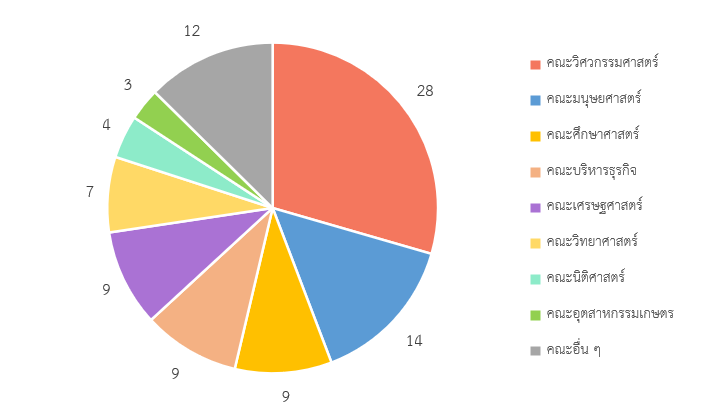
\includegraphics[width=\linewidth]{images/group_by_faculty.png}
  \end{center}
  \caption[จำนวนผู้ตอบแบบสอบถามแบ่งตามคณะที่ศึกษา]{จำนวนผู้ตอบแบบสอบถามแบ่งตามคณะที่ศึกษา}
  \label{fig:faculty}     
\end{figure}

จากการสรุปผลการสำรวจ กราฟที่ \ref{fig:check_before_enrollment} แสดงให้เห็นว่าผู้ตอบแบบสอบถามส่วนใหญ่นั้นตรวจสอบตารางสอบของทุกวิชาที่ต้องการจะลงทะเบียน
ก่อนที่จะลงทะเบียนเรียนอย่างสม่ำเสมอ แต่ยังมีผู้ตอบแบบสอบถามบางส่วนที่ตรวจสอบตารางสอบเพียงบางวิชาก่อนจะลงทะเบียนเรียน และยังมีมีผู้ตอบแบบสอบถามส่วนน้อยที่ตอบว่าไม่เคยตรวจสอบตารางสอบของตนเองเลย
จากกราฟที่ \ref{fig:registration_exam} เรายังพบอีกว่า กลุ่มสำรวจกว่า 80\% ไม่ทราบว่าสำนักทะเบียนและประมวลผล มหาลัยเชียงใหม่ จัดตารางสอบปลายภาคให้กับแต่ละวิชาอย่างไร
\begin{figure}
  \begin{center}
    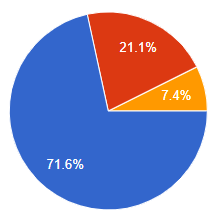
\includegraphics{images/checking_schedule_before_enrollment.png}\\[2ex]
    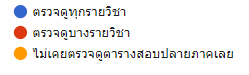
\includegraphics{images/legend_for_checking_schedule_before_enrollment.png}
  \end{center}
  \caption[จำนวนผู้ตอบแบบสอบถามที่ตรวจสอบตารางสอบปลายภาคก่อนการลงทะเบียน]{จำนวนผู้ตอบแบบสอบถามที่ตรวจสอบตารางสอบปลายภาคก่อนการลงทะเบียน}
  \label{fig:check_before_enrollment}     
\end{figure}
\begin{figure}
  \begin{center}
    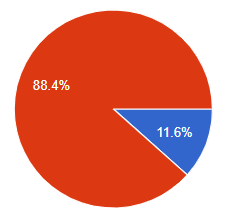
\includegraphics{images/registration_exam.png}\\[2ex]
    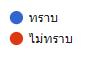
\includegraphics{images/legend_for_registration_exam.png}
  \end{center}
  \caption[จำนวนผู้ตอบแบบสอบถามที่ทราบวิธีการจัดตารางสอบปลายภาคของสำนักทะเบียน]{จำนวนผู้ตอบแบบสอบถามที่ทราบวิธีการจัดตารางสอบปลายภาคของสำนักทะเบียน}
  \label{fig:registration_exam}     
\end{figure}

จากกราฟที่ \ref{fig:time} เราสามารถบอกได้ว่าเวลาที่ผู้ตอบแบบสอบถามส่วนใหญ่ต้องการที่จะสอบในแต่ละวันคือ
ช่วงเวลา 12.00--15.00 ซึ่งผู้ตอบแบบสอบถามส่วนมากต้องการจะสอบช่วงเวลานี้มากกว่า 15.30--18.00 และ 08.00--11.00 ตามลำดับ
\begin{figure}
  \begin{center}
    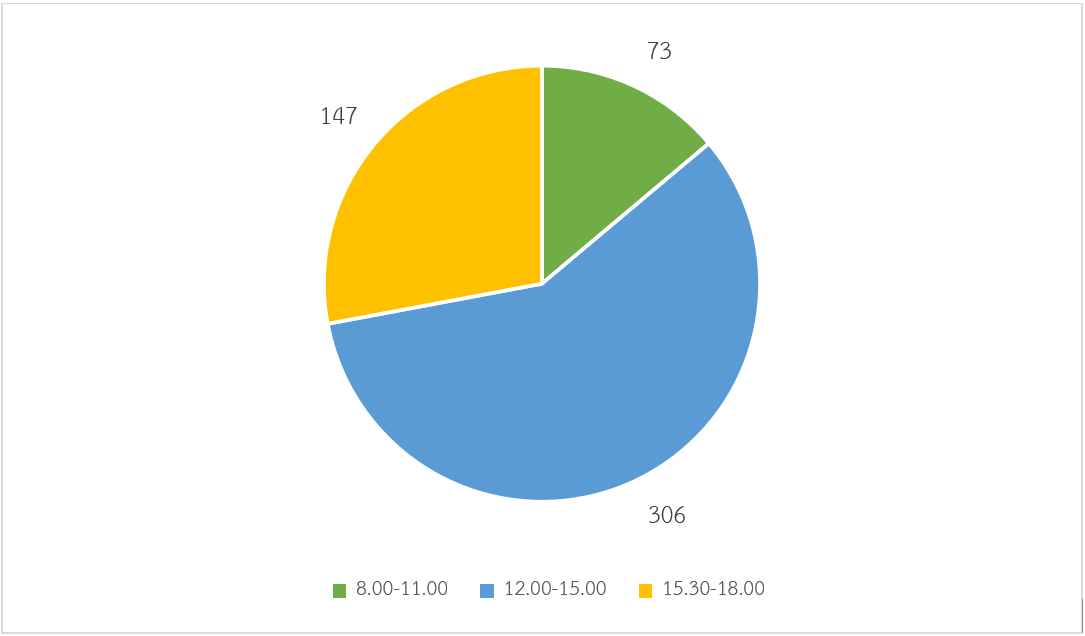
\includegraphics[width=\linewidth]{images/pie_chart_for_final_exam_time.png}
  \end{center}
  \caption{ความต้องการในการสอบของผู้ตอบแบบสอบถามในแต่ละเวลา}
  \label{fig:time}
\end{figure}
และจากกราฟที่ \ref{fig:time_slot} เราทำการรวมช่วงเวลาที่ผู้ตอบแบบสอบถามต้องการสอบกับวันที่ผู้ตอบแบบสอบถามต้องการสอบเข้าด้วยกัน ซึ่งจะสามารถสรุป slot ที่ผู้ตอบแบบสอบถามต้องการจะสอบมากที่สุด 7 อันดับแรก โดยเรียงลำดับจากมากไปน้อยได้ ดังนี้
\begin{figure}
  \begin{center}
    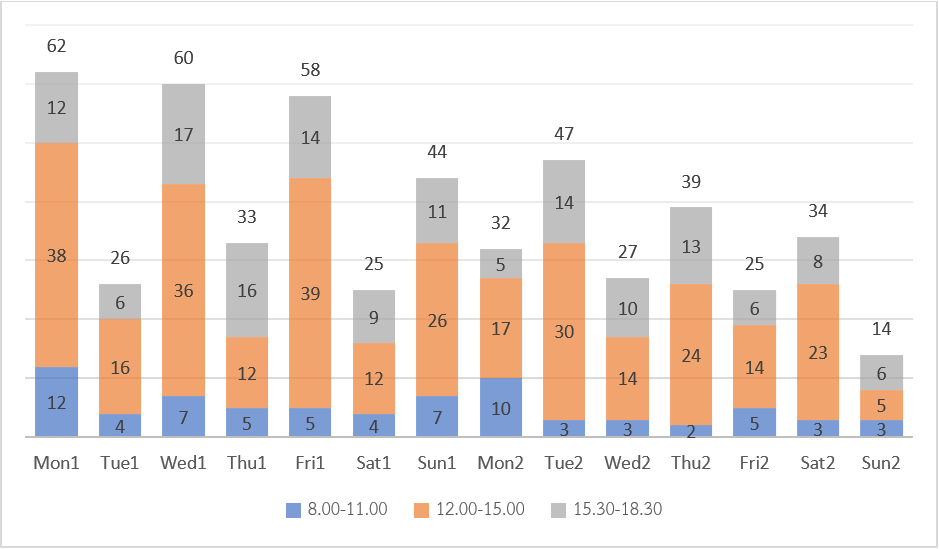
\includegraphics[width=\linewidth]{images/bar_chart_for_final_exam_slot.png}
  \end{center}
  \caption[ความต้องการในการสอบของผู้ตอบแบบสอบถามในแต่ละช่วงเวลาสอบ]{ความต้องการในการสอบของผู้ตอบแบบสอบถามในแต่ละช่วงเวลาสอบ}
  \label{fig:time_slot}     
\end{figure}
\begin{enumerate}
  \item สัปดาห์ที่หนึ่ง เวลา 12.00-15.00น. วันศุกร์ 
  \item สัปดาห์ที่หนึ่ง เวลา 12.00-15.00น. วันจันทร์
  \item สัปดาห์ที่หนึ่ง เวลา 12.00-15.00น. วันพุธ
  \item สัปดาห์ที่สอง เวลา 12.00-15.00น. วันอังคาร
  \item สัปดาห์ที่หนึ่ง เวลา 12.00-15.00น. วันอาทิตย์
  \item สัปดาห์ที่สอง เวลา 12.00-15.00น. วันพฤหัสบดี
  \item สัปดาห์ที่สอง เวลา 12.00-15.00น. วันเสาร์
\end{enumerate}

แต่หากเราตัดเรื่องเวลาที่สอบออก เรายังสามารถสรุปวันที่ผู้ทำแบบสอบถามต้องการจะสอบมากที่สุด 7 อันดับแรก โดยเรียงลำดับจากมากไปน้อย ดังนี้
\begin{enumerate}
  \item สัปดาห์ที่หนึ่ง วันจันทร์
  \item สัปดาห์ที่หนึ่ง วันพุธ
  \item สัปดาห์ที่หนึ่ง วันศุกร์ 
  \item สัปดาห์ที่หนึ่ง วันอาทิตย์
  \item สัปดาห์ที่สอง วันอังคาร
  \item สัปดาห์ที่สอง วันพฤหัสบดี
  \item สัปดาห์ที่สอง วันเสาร์
\end{enumerate}
ซึ่งจากกราฟ \ref{fig:time_slot} ยังสามารถสรุปได้ว่าผู้ตอบแบบสอบถามส่วนใหญ่ต้องการที่จะสอบหนึ่งวันเว้นหนึ่งวันเพื่อที่จะได้มีเวลาในการอ่านหนังสือเตรียมสอบสำหรับวิชาในวันถัดไปมากกว่าการสอบติดกัน 
เรายังสามารถบอกเพิ่มเติมได้อีกว่าผู้ตอบแบบสอบถามส่วนใหญ่ต้องการสอบในช่วงสัปดาห์แรกของช่วงการสอบมากกว่าช่วงสัปดาห์ที่สองเพื่อที่จะได้มีเวลาพักผ่อนหรือกลับบ้าน หลังจากที่สอบเสร็จแล้ว

\subsection{การเก็บข้อมูลตารางสอบ}
หลังจากได้ผลการสำรวจแล้วเราจึงได้ออกสำรวจเพื่อเก็บข้อมูลรายวิชาต่าง ๆ ที่มีการจัดสอบจากแต่ละคณะ โดยได้ทำคำร้องขอข้อมูลไปยังแต่ละคณะ ซึ่งข้อมูลที่ต้องการใช้งาน ได้แก่ ข้อมูลห้องที่สามารถจัดสอบได้ พร้อมจำนวนนักศึกษาที่จุได้ในแต่ละห้องของแต่ละคณะ
และข้อมูลตารางสอบปลายภาคของแต่ละคณะ เป็นเวลา 3 ปี ย้อนหลัง ซึ่งทางเราได้ตั้งสมมติฐานว่า วิชาใดที่มีรายชื่อวิชาอยู่ในคำสั่งแต่งตั้งกรรมการคุมสอบของแต่ละคณะนั้น จะมีการจัดสอบปลายภาคจริง ๆ
โดยมีตัวอย่างใบบันทึกข้อความเพื่อขอข้อมูลดังที่ได้กล่าวมา ดังรูปที่ \ref{fig:request-memo-scan}
\begin{figure}
  \begin{center}
    
\includegraphics[width=\linewidth]{images/request_memo_scan.png}
  \end{center}
  \caption[ตัวอย่างใบบันทึกข้อความเพื่อขอข้อมูลตารางสอบ]{ตัวอย่างใบบันทึกข้อความเพื่อขอข้อมูลตารางสอบ}
  \label{fig:request-memo-scan}     
\end{figure}
\CIreply{ใส่รูปสแกนบันทึกข้อความของสักคณะ}

\section{โครงสร้างและการทำงานของโปรแกรม}

\subsection{รูปแบบของผลลัพธ์จากการจัดตารางสอบ}
ข้อมูลผลลัพธ์ของโปรแกรมจะเป็นไฟล์ CSV ที่ระบุรายวิชาคู่กับหมายเลข slot ที่สอบของรายวิชานั้น ๆ โดยจะมีข้อมูลใช้สำหรับ mapping หมายเลข slot เป็นวันและเวลาสอบ
โดยหมายเลข slot แต่ละหมายเลขจะบ่งบอกถึงวันและเวลาสอบที่ต่างกันในแต่ละภาคการศึกษา

\subsection{การออกแบบอัลกอริทึมและแผนผังการทำงานของโปรแกรม}
ในการออกแบบอัลกอริทึมสำหรับใช้ในการจัดตารางสอบ จะใช้วิธีการระบายสีกราฟ (graph coloring) 
โดยจะแปลงรายวิชาที่ต้องจัดสอบเป็นโหนดของกราฟ (node) 
และคู่วิชาที่มีนักศึกษาคนใด ๆ ลงทะเบียนพร้อมกันในภาคการศึกษานั้นจะถูกจัดให้สอบพร้อมกันไม่ได้ 
จึงจะถูกแปลงเป็นเส้นเชื่อมในกราฟ (edge) จำนวนนักศึกษาที่ลงทะเบียนในคู่วิชานั้น ๆ จะถูกแปลงเป็น edge weights
และช่วงเวลาที่แต่ละวิชาจัดสอบ (slot) จะถูกแปลงเป็นสีของโหนด
สำหรับแต่ละโหนด เราจะนิยาม \emph{degree of conflicts} เป็นผลรวมของ weights จากทุกๆ edge ที่ต่ออยู่กับโหนดนั้นๆ
และเรียกจำนวนเส้นเชื่อมทั้งหมดที่เข้า--ออก จากกราฟว่า\emph{ดีกรี} (degree) 
โดยอัลกอริทึมจะมีลำดับการทำงานตามรูปที่ \ref{fig:flowchart} 
โดยเมื่อจะรันโปรแกรมจะต้องเลือกอัลกอริทึมรูปแบบใดรูปแบบหนึ่ง จากทั้งหมด 4 รูปแบบ ดังขั้นตอนที่ 1
และอัลกอริทึมจะมีรูปแบบการทำงานทั้งหมด 4 รูปแบบ โดยแต่ละรูปแบบจะมีความแตกต่างกันที่ลำดับการเลือกโหนดมาเพื่อละบายสี
โดยแต่ละรูปแบบจะมีการเรียงลำดับ ดังตอนที่ \ref{subsec:sorting_type}

\subsection{รูปแบบของอัลกอริทึม}
\label{subsec:sorting_type}
\begin{enumerate}
  \item รูปแบบที่ 1 BFS-DEG: ทำ BFS จากแต่ละโหนดโดยมีการเรียงลำดับความสำคัญของโหนดที่จะจัดช่วงเวลาสอบก่อน โดยเรียงจาก
  ดีกรีของโหนด จำนวนนักศึกษาที่ลงทะเบียน จำนวน conflict ของโหนด และหากทุกอย่างเท่ากันจะเรียงตามรหัสวิชา โดยเรียงจากมากไปน้อยตามลำดับ
  เมื่อจัดช่วงเวลาสอบให้ครบทุกโหนดเพื่อนบ้านแล้วจะเริ่มกระบวนการนี้ซ้ำที่โหนดเพื่อนบ้านถัดไป จนกว่าจะจัดช่วงเวลาสอบได้ครบทุกโหนด
  \item รูปแบบที่ 2 DEG: จัดช่วงเวลาสอบให้แต่ละโหนดโดยมีการเรียงลำดับความสำคัญของโหนดที่จะจัดช่วงเวลาสอบก่อน โดยเรียงจาก
  ดีกรีของโหนด จำนวนนักศึกษาที่ลงทะเบียน จำนวน conflict ของโหนด และหากทุกอย่างเท่ากันจะเรียงตามรหัสวิชา โดยเรียงจากมากไปน้อยตามลำดับ
  \item รูปแบบที่ 3 BFS-STD: ทำ BFS จากแต่ละโหนดโดยมีการเรียงลำดับความสำคัญของโหนดที่จะจัดช่วงเวลาสอบก่อน โดยเรียงจาก
  จำนวนนักศึกษาที่ลงทะเบียน ดีกรีของโหนด จำนวน conflict ของโหนด และหากทุกอย่างเท่ากันจะเรียงตามรหัสวิชา โดยเรียงจากมากไปน้อยตามลำดับ
  เมื่อจัดช่วงเวลาสอบให้ครบทุกโหนดเพื่อนบ้านแล้วจะเริ่มกระบวนการนี้ซ้ำที่โหนดเพื่อนบ้านถัดไป จนกว่าจะจัดช่วงเวลาสอบได้ครบทุกโหนด
  \item รูปแบบที่ 4 STD: จัดช่วงเวลาสอบให้แต่ละโหนดโดยมีการเรียงลำดับความสำคัญของโหนดที่จะจัดช่วงเวลาสอบก่อน โดยเรียงจาก
  จำนวนนักศึกษาที่ลงทะเบียน ดีกรีของโหนด จำนวน conflict ของโหนด และหากทุกอย่างเท่ากันจะเรียงตามรหัสวิชา โดยเรียงจากมากไปน้อยตามลำดับ
\end{enumerate}

\CIreply{เรายังต้องทำตาม component จริงหรือ? หรือแค่ทำจนครบทุก node เรียงลำดับตามวิธีที่เราเลือกใช้?}
\TSNAreply{ถ้าใช้ BFS ต้องแยก component เพราะไม่งั้นจะ visit ไม่ครบทุก node แต่ถ้าไม่ใช้ BFS น่าจะไม่ต้องตาม component ได้ครับ}
\begin{figure}
  \begin{center}
    \begin{tikzpicture}[flowchart]
      \node[startstop] (start) {start};
      \node[io] (a) [below=0.4cm of start] {{เลือกรูปแบบการทำงานของอัลกอริทึมจากทั้งหมด 4 รูปแบบ}};
      \node[io2] (b) [below=0.4cm of a] {{
        \begin{minipage}{4.25in}
        \begin{itemize}[nosep]
        \item อ่านข้อมูลลงทะเบียนของนักศึกษาแต่ละคน
        \item อ่านข้อมูลรายวิชาทั้งหมดที่มีนักศึกษาลงทะเบียน
        \item อ่านข้อมูลคู่รายวิชาที่มีนักศึกษาลงทะเบียนทั้งสองวิชาอย่างน้อย 1 คน (conflicts)
        \item อ่านข้อมูลรายวิชาทั้งหมดที่มีการจัดสอบ
        \item อ่านข้อมูลรายวิชาของแต่คณะ
        \item อ่านข้อมูลจำนวนความจุของที่นั่งสอบของแต่ละคณะ
      \end{itemize}        
      \end{minipage}    
      }};
      \node[process] (proa) [below=0.4cm of b ] {
        \begin{minipage}{3.6in}
          คัดกรองรายวิชาที่ต้องจัดสอบให้เหลือเพียงรายวิชาที่มีนักศึกษาลงทะเบียนและเป็นรายวิชาที่มีอยู่ในลิสต์ของรายวิชาที่มีการจัดสอบ
        \end{minipage}    
        };
      \node[process] (prob) [below=0.4cm of proa] {
      \begin{minipage}{3.7in}
        สร้างกราฟ
        \begin{itemize}[nosep]
        \item เพิ่ม nodes ของกราฟจากรายวิชาที่ได้จากขั้นตอนก่อนหน้า
        \item เพิ่ม edges ของแต่ละ nodes ตามคู่รายวิชาที่มี conflicts
      \end{itemize}        
      \end{minipage}                      
      };
      \node[process] (proc) [below=0.4cm of prob] {แยกกราฟย่อยออกจากกราฟตาม connected component};
      \node[connector] (con) [below=0.4cm of proc] {};
      \node[decision] (desa) [below=0.4cm of con] {visit ครบทุก component?};
      \node[process] (prod) [below=0.4cm of desa] {visit component ถัดไป};
      \node[process] (proe) [below=0.4cm of prod] {
        \begin{minipage}{4.3in}
          จัดตารางสอบให้แต่ละ node โดยการเลือก slot สอบตาม penalty model โดยการทดลองทุก slot ที่จัดสอบได้และเลือก slot ที่ทำให้ค่า penalty น้อยที่สุด โดยจะจัด slot สอบให้แต่ละ node เรียงตามรูปแบบของอัลกอริทึมที่เลือก
        \end{minipage} 
      };
      \node[process] (prof) [below=0.2cm of proe] {คิดคำนวณค่า penalty ของตารางสอบ};
      \node[io] (c) [below=0.4cm of prof] {
        \begin{minipage}{3.7in}
          \begin{itemize}[nosep]
          \item แสดงค่า penalty ของตารางสอบ
          \item เขียนผลลัพธ์ของตารางสอบและค่า penalty ลงในไฟล์
        \end{itemize}        
        \end{minipage}  };
      \node[startstop] (end) [below=0.4cm of c] {end};
      
      \draw[arrow] (start) -- (a);
      \draw[arrow] (a) -- (b);
      \draw[arrow] (b) -- (proa);
      \draw[arrow] (proa) -- (prob);
      \draw[arrow] (prob) -- (proc);
      \draw[arrow] (proc) -- (con);
      \draw[arrow] (con) -- (desa);
      \draw[arrow] (proc) -- (con);
      \draw[arrow] (desa) -- node[near start,right]{False} (prod);
      \draw[arrow] (desa.east) -- node[near start,above]{True} +(3.5cm,0) |- (prof);
      \draw[arrow] (prod) -- (proe);
      \draw[arrow] (proe.west) -- +(-0.5cm,0) |- (con);
      \draw[arrow] (prof) -- (c);
      \draw[arrow] (c) -- (end);
            
    \end{tikzpicture}
  \end{center}
  \caption[แผนผังการทำงานของโปรแกรม]{แผนผังการทำงานของโปรแกรม}
  \label{fig:flowchart}     
\end{figure}

